% The Levenshtein automaton for the word "cat" at distance ≤ 1 (Schulz–Mihov): a
% trellis of states (i, e) = (position in the word, errors so far). Match edges
% (solid teal, cost 0) read the word's char; edit edges (amber, cost 1) are
% insertion (↑), substitution (↗), and deletion (ε, dashed). Accepting = the
% rightmost column (i = 3), any e ≤ 1.
\documentclass[border=10pt]{standalone}
\usepackage{tikz}
\usetikzlibrary{arrows.meta, positioning}
\usepackage{xcolor}
\definecolor{matchc}{HTML}{0D9488}
\definecolor{editc}{HTML}{D97706}
\definecolor{accc}{HTML}{16A34A}
\begin{document}
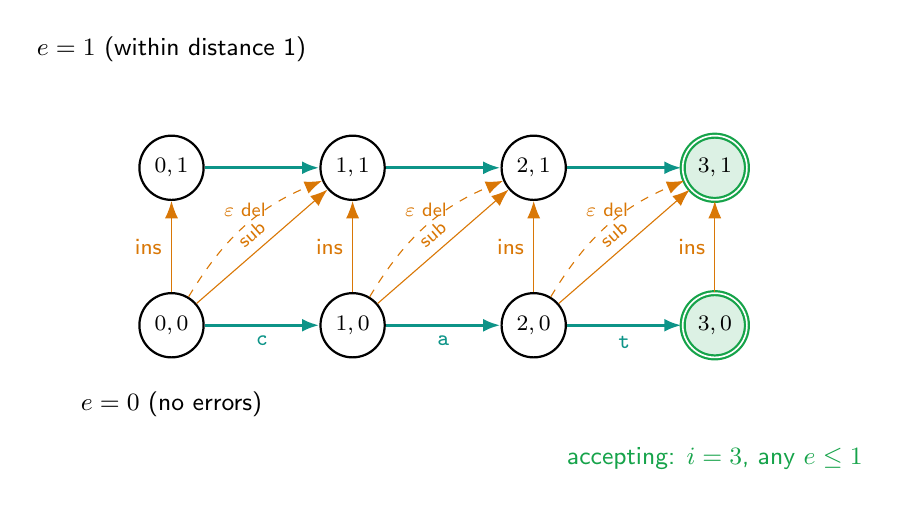
\begin{tikzpicture}[
    >={Latex[length=2.2mm]},
    st/.style={circle, draw, thick, minimum size=8mm, font=\sffamily\footnotesize},
    acc/.style={st, double, fill=accc!15, draw=accc},
    every node/.style={font=\sffamily\footnotesize},
    x=2.3cm, y=2.0cm]

  % rows: e = 0 (bottom), e = 1 (top); columns i = 0..3
  \foreach \i in {0,1,2,3} {
    \node[st] (e0-\i) at (\i,0) {$\i,0$};
  }
  \node[acc] (e0-3) at (3,0) {$3,0$};   % redraw accepting
  \foreach \i in {0,1,2,3} {
    \ifnum\i=3 \node[acc] (e1-\i) at (\i,1) {$\i,1$};
    \else \node[st] (e1-\i) at (\i,1) {$\i,1$}; \fi
  }

  % match edges (read the word char, cost 0) along each row
  \foreach \i [evaluate=\i as \j using int(\i+1)] in {0,1,2} {
    \draw[->, matchc, very thick] (e0-\i) -- (e0-\j) node[midway, below, matchc]{\ttfamily \ifcase\i c\or a\or t\fi};
    \draw[->, matchc, very thick] (e1-\i) -- (e1-\j);
  }
  % insertion edges (↑, any char, +1 error)
  \foreach \i in {0,1,2,3} {
    \draw[->, editc] (e0-\i) -- (e1-\i) node[midway, left, editc]{ins};
  }
  % substitution edges (↗, any char, +1 error)
  \foreach \i [evaluate=\i as \j using int(\i+1)] in {0,1,2} {
    \draw[->, editc] (e0-\i) -- (e1-\j) node[midway, sloped, above, editc, font=\sffamily\scriptsize]{sub};
  }
  % deletion edges (ε, skip a word char, +1 error) — dashed
  \foreach \i [evaluate=\i as \j using int(\i+1)] in {0,1,2} {
    \draw[->, editc, dashed] (e0-\i) to[bend left=18] node[midway, above, editc, font=\sffamily\scriptsize]{$\varepsilon$ del} (e1-\j);
  }

  \node[below=3mm of e0-0, font=\sffamily\small] {$e=0$ (no errors)};
  \node[above=8mm of e1-0, font=\sffamily\small] {$e=1$ (within distance 1)};
  \node[below=10mm of e0-3, accc, font=\sffamily\small] {accepting: $i=3$, any $e\le 1$};
\end{tikzpicture}
\end{document}
